\documentclass[twocolumn, a4paper, 12pt]{article}
\usepackage{graphicx} % Required for inserting images
\graphicspath{{./images/}}
\usepackage{float}  % For [H] option to control figure placement
\usepackage[
backend=biber,
style=numeric,
sorting=ynt
]{biblatex}
\addbibresource{references.bib}

\title{The Role of Education and Emotion in Spreading Misinformation across Social Networks: An Agent Based Modelling Approach}
\author{Ahmed Abdelhaleem \\ University of Sussex}
\date{January 2025}

\begin{document}

\maketitle


\begin{abstract}
  This study explores the dynamics of misinformation spread in social networks using agent based modelling (ABM), focusing on two key parameters: education and emotion. The model simulates agents with varying educational backgrounds and emotional states to assess how these factors influence susceptibility to misinformation across different socio emotional classes. Education is treated as a logic parameter, with agents possessing varying levels of media literacy and critical thinking skills. Emotion, as the second parameter, examines the impact of emotional triggers like anger, on belief in misinformation. Trust, as the third parameter, combines as both a logic and an emotional parameter. By integrating these factors, the model aims to provide insights into how misinformation spreads differently across various socio emotional classes. This research aims to offer a better understanding of the socio emotional mechanisms behind misinformation and inform strategies to counteract its spread.
\end{abstract}

\tableofcontents   % Table of Contents
\listoffigures     % Table of Figures


\section{Introduction}
Misinformation is a pervasive issue in today's digital age, with far reaching effects on individuals, communities, and societies. Social media platforms and online networks serve as primary vehicles for the spread of misinformation, amplifying its reach and impact.

Misinformation is defined as incorrect information, and it is possible for this information to be made incorrect by accident, not particularly intentional. One such example of that would be to spread an old outdated story.\cite{definition}

Previous published research, has indicated that both cognitive and emotional factors play significant roles in misinformation dissemination. Education, and emotional states such as anger can affect how individuals process and share information \cite{education} \cite{emotion}. However, there is limited understanding of how these factors interact across different socio emotional classes.

However, the trust parameter in this research uses a novel approach, through examining it as both an emotional and a logical parameter simultaneously, a technique that has not been thoroughly explored in prior studies. Trust is often treated as a purely emotional parameter or, conversely, as a rational parameter based on logical thinking and reasoning. However, in a real world scenario, trust operates at the intersection of these two domains, influenced by both emotional reactions and logical reasoning. By integrating trust into the model as a dual faced parameter, this research aims to capture its unique role in shaping human behaviour, particularly in the context of misinformation spread and fact checking.

This approach provides a more holistic understanding of trust's impact on decision making, bridging the gap between emotional and cognitive dimensions, and offering fresh insights into its influence in misinformation spread and hoax checking.

This research models a misinformation spread system using an agent based modelling (ABM) approach, to try and investigate the intersection between education, emotion, and misinformation spread in social networks, focusing heavily on how these dynamics differ across socio emotional classes. Understanding these factors can help in designing targeted interventions to combat the spread of misinformation or at least mitigate it by a certain percentage.

In the results and analysis, multiple key metrics will be evaluated, including misinformation spread rate, belief contagion, the credibility score of a hoax, and the impact of education and emotion, through simulations under varying parameter settings, such as different education levels or emotional triggers, through varying the percentages of different socio emotional classes found in the social network system. The aim of the following analyses is to try and uncover patterns or thresholds that strongly influence the dynamics of misinformation spread in social network systems.

In the discussion section, the uncovered findings will be linked to the following research questions: How do education and emotion interact to affect misinformation spread? and what interventions could effectively mitigate the spread of misinformation in the social network system? This structured approach ensures perfect alignment with the project objectives.



\section{Methods}
An agent based model was created to simulate the behaviour of agents within a social network. Each agent in the model represents a person, with parameters for education level, emotional state, and socio emotional class. These parameters influence how agents interact with information and each other, particularly in relation to misinformation. The model simulates the following:

• Education: Agents have varying levels of education, from low to high, which
influences their critical thinking and their ability to verify information.

• Emotion: Agents have varying levels of emotional states, from low to high; examples of emotional states (e.g. anger) affect their likelihood to believe or spread misinformation.

• Socio emotional Class: Agents are categorized into different socio emotional groups based on factors like access to education, which may impact their exposure to misinformation and emotional responses.

In this study, socio emotional classes were introduced to model the interplay between the varying emotional states and education levels in the spread of misinformation. Four distinct classes were defined to capture all possible combinations: (1) High Emotional, High Education, (2) High Emotional, Low Education, (3) Low Emotional, High Education, and (4) Low Emotional, Low Education. These classes represent a wide range of socio emotional profiles, with the emotional parameter increasing the agent's susceptibility to believing misinformation and potentially spreading it afterwards and the educational parameter increasing their tendency to fact check.

Each agent in the simulation was randomly assigned to one of these classes, determining their respective levels of anger, education, and trust. The emotional parameter anger modulated the probability of transitioning to a believer state, while the educational parameter increased the likelihood of becoming a fact checker.

This classification allowed for a nuanced representation of heterogeneous behaviours within the network, ensuring that the model realistically reflected the diversity of socio emotional factors in a population.

\subsection{Used Model and Parameters}
The "SBFC" model \cite{simulation} was used in this research, which stands for \textbf{S}usceptible, \textbf{B}eliever, and \textbf{F}act \textbf{C}hecker. This "SBFC" model was implemented in the Python programming language using the "NetworkX" library, to simulate the social network of agents and their connections with each other.

The social network was represented by a normal graph using the "NetworkX" library, where each node represents an agent of the system, and each edge represents a connection or a friendship between 2 agents.

The verification probability parameter "pv" is responsible for transforming a believer into a fact checker, and the forgetting probability parameter "pf" is responsible for making a fact checker or believer agent to forget and return to becoming suspensible.

Initially, 90\% of all agents are susceptible, and the rest of the 10\% are believers. There are two equations governing the change of an agent state from susceptible to believer or fact checker, which can be seen in Equation \ref{eq:1} and Equation \ref{eq:2}.

In the paper, the conditions for transitioning from Susceptible (S) to either Believer (B) or Fact Checker (FC) are based on the spreading functions $f_B^i$ and $f_{FC}^i$, which can be seen in Equation \ref{eq:1} and Equation \ref{eq:2}. \cite{simulation} Here's the exact workflow:

Transition from $S$ to $B$ or $FC$:

1. A Susceptible agent becomes:

   - A Believer (B) with probability $f_B^i$, the spreading function for Believers.
   
   - A Fact Checker (FC) with probability $f_{FC}^i$, the spreading function for Fact Checkers.

2. The spreading functions are defined as:
   \begin{equation} \label{eq:1}
   f_B^i(t) = \beta \cdot \frac{n_B^i(t) \cdot (1 + \alpha)}{n_B^i(t) \cdot (1 + \alpha) + n_{FC}^i(t) \cdot (1 - \alpha)}
   \end{equation} \cite{simulation}

   \begin{equation} \label{eq:2}
   f_{FC}^i(t) = \beta \cdot \frac{n_{FC}^i(t) \cdot (1 - \alpha)}{n_B^i(t) \cdot (1 + \alpha) + n_{FC}^i(t) \cdot (1 - \alpha)}
   \end{equation} \cite{simulation}
   
   - where $n_B^i(t)$: Number of neighbours of node $i$ in state $B$ (Believer).
   
   - $n_{FC}^i(t)$: Number of neighbours of node $i$ in state $FC$ (Fact Checker).
   
   - $\alpha$: Credibility of the hoax.
   
   - $\beta$: Spreading rate.

I modelled the education parameter for an agent to have an inverse relation with believing the misinformation and a direct relation with fact checking this misinformation, i.e. when the education of a certain agent increases, the belief factor decreases and the fact checking factor increases. \cite{education}

\subsection{Parameter Modifications}
I modelled the anger parameter for an agent to have an inverse relation with fact checking the misinformation and a direct relation with believing this misinformation, i.e. when the anger of a certain agent increases, the belief factor increases, and the fact checking factor decreases. \cite{emotion}

The trust parameter is multiplied by the number of neighbours of a certain state (Believer or Fact Checker) and added to the $f_{FC}$ or $f_B$ functions respectively. To see the effect of the modelled trust parameter clearly, every agent in the social network have a 10\% of the total network as its neighbours and is connected through an edge.

Instead of giving a fixed value for the Verification Probability (pv), it is now dependent on the education, anger, and anger parameters of each agent.

\subsection{Simulation Environment}
The simulation was run on a network of agents with a fixed degree of connection, mimicking social media interactions. Agents can interact with each other by sharing information (true or false), and each interaction has a probability of changing the agent’s beliefs based on the interaction’s emotional intensity and the agent’s education level.

\subsection{Metrics}
The key outcome metrics of the model include:

• Misinformation Spread Rate $\beta$: The proportion of agents who believe and
subsequently share misinformation.

• Belief Contagion: The number of connections or interactions through which
misinformation spreads.

• Impact of Education and Emotion: The correlation between agent's education
levels, emotional responses, and the likelihood of adoption and sharing of misinformation.

\section{Results and analyses}
\subsection{Experiment Parameters}
Different percentages of socio emotional classes were tested in this model, with varying levels of hoax credibility $\alpha$, these results with varying parameters will be analysed to identify the misinformation spread thresholds.

In the context of the misinformation spread model presented in the cited paper \cite{simulation}, $\alpha$ represents the credibility of the hoax. It is a parameter that influences the likelihood of an agent believing the misinformation versus its debunking. Viewing its impact:

- High $\alpha$ (0.8): The hoax is perceived as highly credible, giving it an advantage in spreading over its debunking.

- Low $\alpha$ (0.3): The hoax is less credible, making it easier to be debunked than to spread.

A forgetting probability "pf" of 0.2 was used all over the tests done. When it is stated that a high value of $\alpha$ is used, it refers to a value of 0.8, while a low value of $\alpha$ corresponds to a value of 0.3. A high education or emotional, means a value of 0.7 for both parameters, and a low value is 0.3. With the trust parameter taking the mean of those 2 parameters.

The below results will show the percentage of each agent state (susceptible, believer, and fact checker) in the whole social network after the end of the simulation, and a graph of those percentages over 200 simulation steps, which represents our time parameter here. In addition to the hoax credibility value used, and the percentage of each socio emotional class.

\subsection{Experiments and analyses}
Firstly, starting with random allocation of the socio emotional classes, with varying the hoax credibility $\alpha$ value.

When the low value of hoax credibility $\alpha$ was used with random placement of the socio emotional classes. Most of the social network agents became believers with a percentage of 73\%, with the percentages of fact checkers dropping to only 4.5\%, and the remaining 22\% was for the susceptible state, as can be seen in Figure \ref{fig:1}.

\begin{figure}[H]
    \centering
    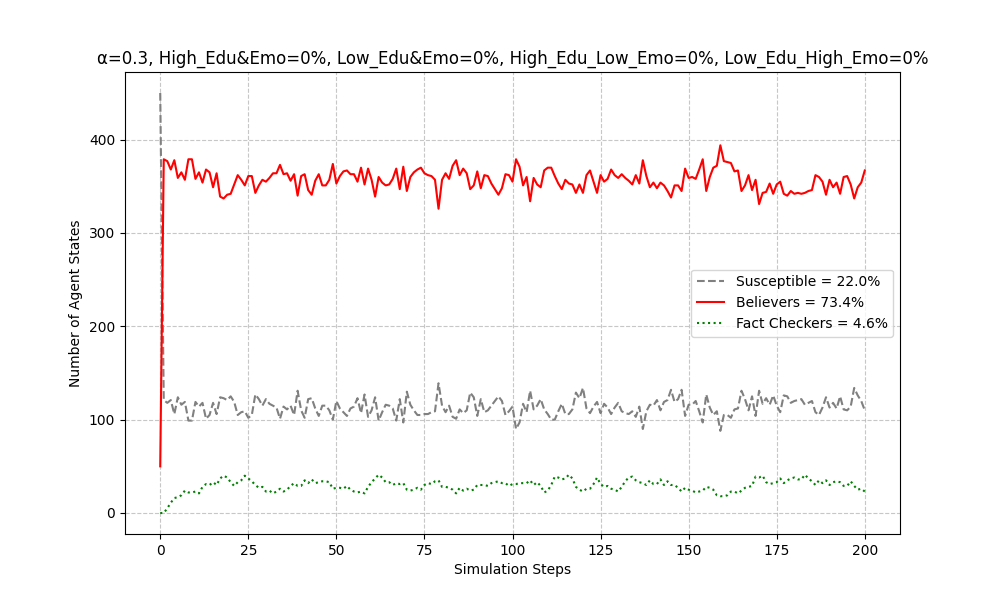
\includegraphics[width=1\linewidth]{0.3_alpha_random.png}
    \caption{Random Classes, $\alpha$=0.3}
    \label{fig:1}
\end{figure}

Using the high value of hoax credibility $\alpha$. Most of the social network agents became believers with a percentage of approximately 65\%, with the percentages of fact checkers being 13\%, and the remaining 22\% was for the susceptible state, as can be seen in Figure \ref{fig:2}.

\begin{figure}[H]
    \centering
    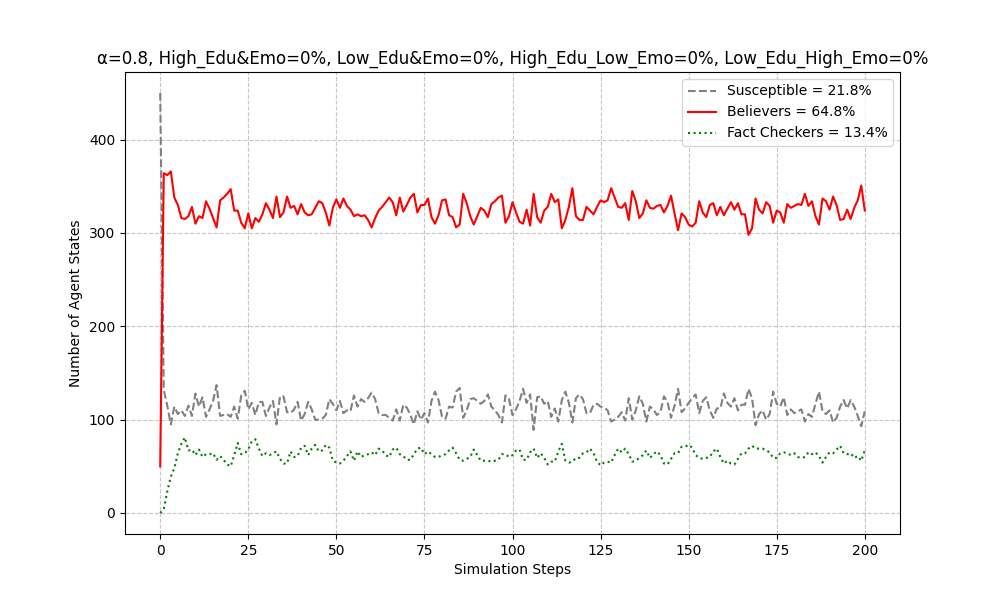
\includegraphics[width=1\linewidth]{0.8_alpha_random.png}
    \caption{Random Classes, $\alpha$=0.8}
    \label{fig:2}
\end{figure}

A slight decrease in the percentage of believers is noticed, when increasing the $\alpha$ value from 0.3 to 0.8, while these results does not align with the expected results from the equations in the cited paper \cite{simulation}. This can be explained by the change in the verification probability "pv" value (controls the change from believer to fact checker), as it now depends on the hoax credibility $\alpha$ and the agent's logical and emotional parameters, instead of having a fixed value.

Secondly, testing with extreme values for the socio emotional classes with varying levels of hoax credibility $\alpha$, to make sure that the model's results aligns with the equations in the cited paper \cite{simulation}.

When the low value of hoax credibility $\alpha$ was used with 100\% of the socio emotional classes being of high education and low emotion. Most of the social network agents became fact checkers, with the percentages of believers dropping down to 0\%, and the remaining percentage was for the susceptible state, as can be seen in Figure \ref{fig:3}.

\begin{figure}[H]
    \centering
    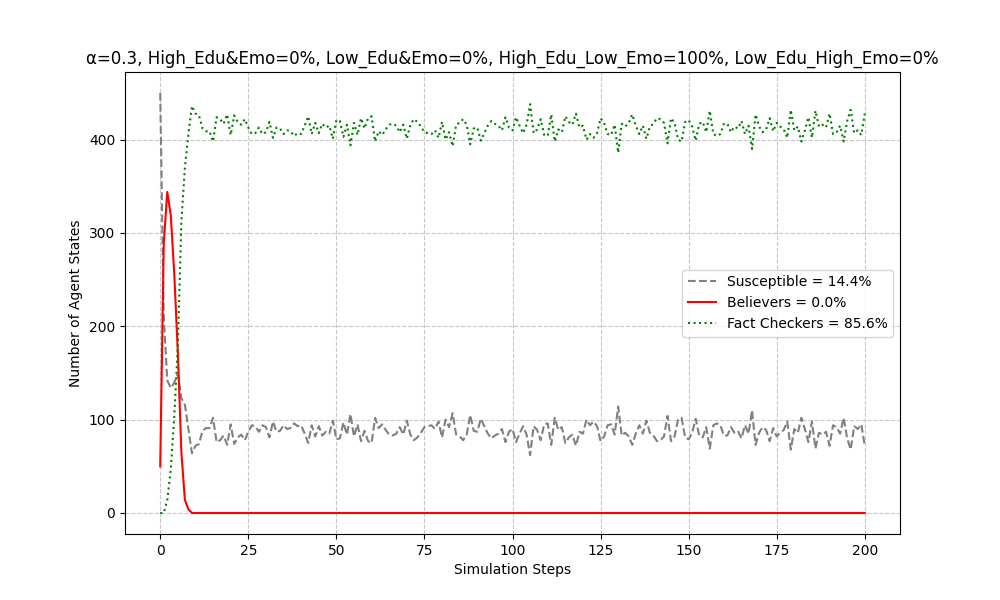
\includegraphics[width=1\linewidth]{0.3_alpha_high.png}
    \caption{High Education \& Low Emotion, $\alpha$=0.3}
    \label{fig:3}
\end{figure}

When the high value of hoax credibility $\alpha$ was used with 100\% of the socio emotional classes being of high education and low emotion. Most of the social network agents became fact checkers, with the percentages of believers dropping down to 0\%, and the remaining percentage was for the susceptible state, as can be seen in Figure \ref{fig:4}.

\begin{figure}[H]
    \centering
    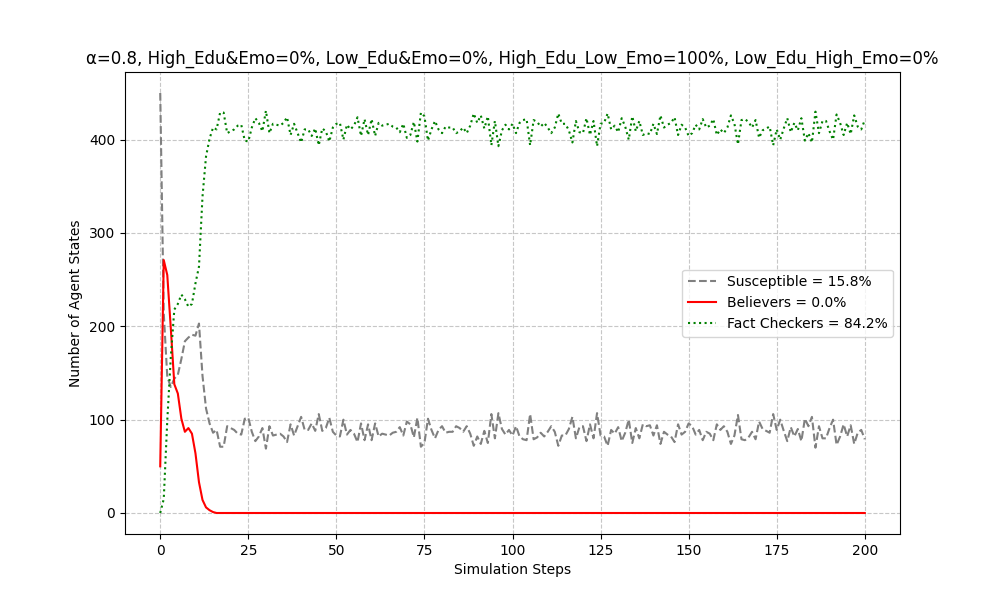
\includegraphics[width=1\linewidth]{0.8_alpha_high.png}
    \caption{High Education \& Low Emotion, $\alpha$=0.8}
    \label{fig:4}
\end{figure}

When the low value of hoax credibility $\alpha$ was used with 100\% of the socio emotional classes being of low education and high emotion. Most of the social network agents became believers, with the percentages of fact checkers dropping down to 0\%, and the remaining percentage was for the susceptible state, as can be seen in Figure \ref{fig:5}. It is worth mentioning that the believers in this test was lower by 3\% as a result of using a lower $\alpha$.

\begin{figure}[H]
    \centering
    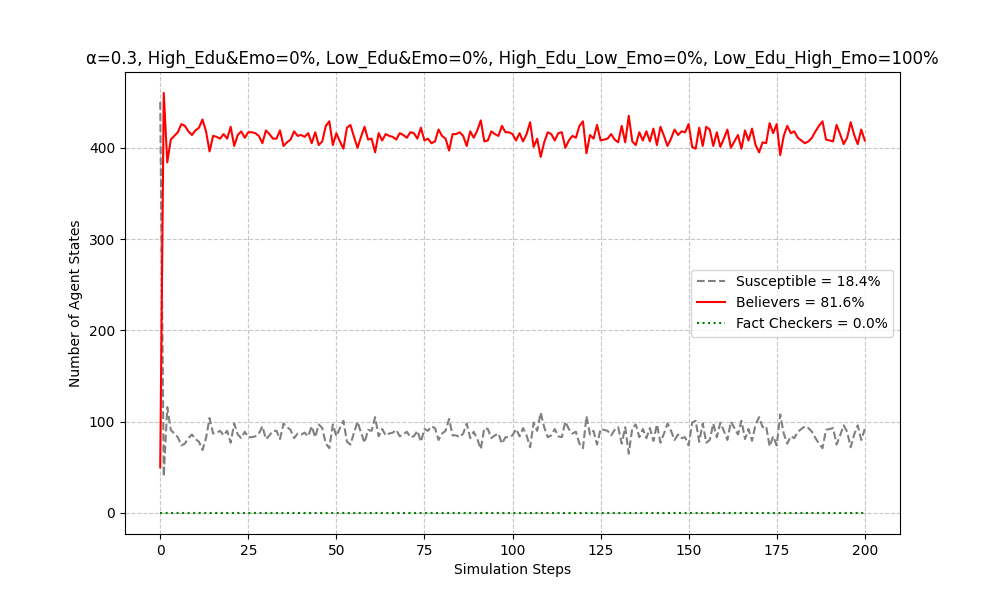
\includegraphics[width=1\linewidth]{0.3_alpha_low_edu.png}
    \caption{Low Education \& High Emotion, $\alpha$=0.3}
    \label{fig:5}
\end{figure}

When the high value of hoax credibility $\alpha$ was used with 100\% of the socio emotional classes being of low education and high emotion. Most of the social network agents became believers, with the percentages of fact checkers dropping down to 0\%, and the remaining percentage was for the susceptible state, as can be seen in Figure \ref{fig:6}.

\begin{figure}[H]
    \centering
    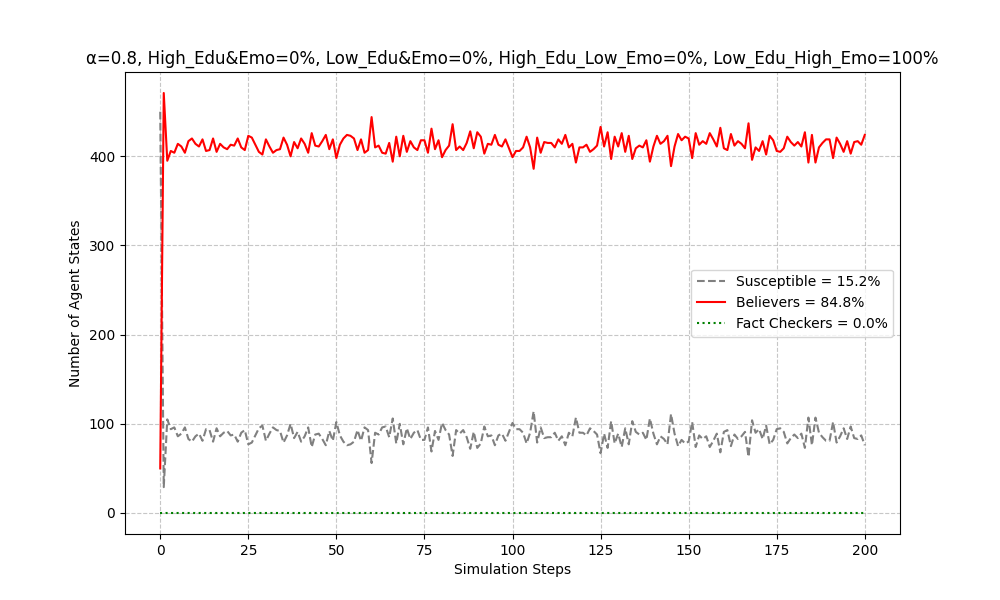
\includegraphics[width=1\linewidth]{0.8_alpha_all_low.png}
    \caption{Low Education \& High Emotion, $\alpha$=0.8}
    \label{fig:6}
\end{figure}


It is very clear that when all the social network consists of high education agents with low emotional parameters, the fact checkers in the network skyrocket and the number of believers fall down to zero. While the opposite is also true, in a social network that consists of low education agents with high emotional parameters.

Running the network with all agents having the same level of education and emotional parameters with both values of hoax credibility $\alpha$, results in the whole network being believers, which aligns with the expected results, as the network only has believers at the start, and no fact checkers, and the equal level of education and emotions cancel each other out, resulting in spreading the hoax and no fact checking occurring.

The results shown here aligns with the expected results from the equations and research in the cited papers \cite{simulation} \cite{emotion} \cite{education}.

Thirdly, as this research aims to mitigate or in an ideal scenario completely stop the spread of misinformation, different percentages of socio emotional classes have been tested to identify the minimum threshold for the high education with low emotional state class, after which the system becomes mostly hoax believers and susceptible agents.

It has been observed that when using a low hoax credibility value (0.3), the minimum percentage for the high education with low emotional state class needs to be at least 63\%, for the system to be mostly fact checkers and prevent it from becoming populated with misinformation believers, as can be seen in Figure \ref{fig:7}.

\begin{figure}[H]
    \centering
    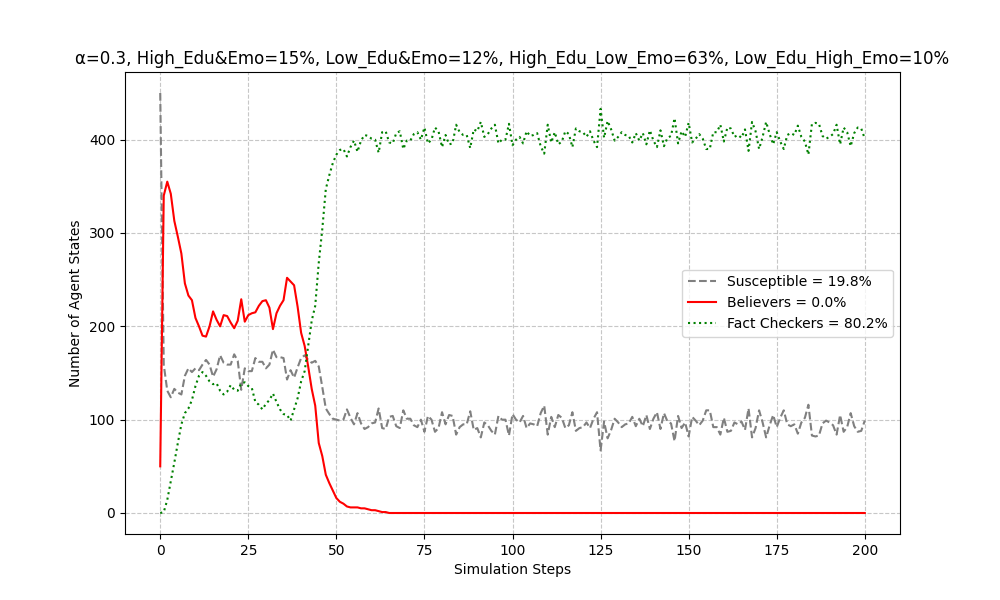
\includegraphics[width=1\linewidth]{min_threshold_fact_checkers.png}
    \caption{Minimum threshold for fact checking, $\alpha$=0.3}
    \label{fig:7}
\end{figure}

Conversely, for a high hoax credibility value (0.8), a higher minimum would be expected, as a higher hoax credibility value increases the probability for any agent to become a believer than a fact checker. The minimum percentage for the high education with low emotional state class needs to be at least 80\%, for the system to have more fact checkers than hoax believers, as can be seen in Figure \ref{fig:8}.

\begin{figure}[H]
    \centering
    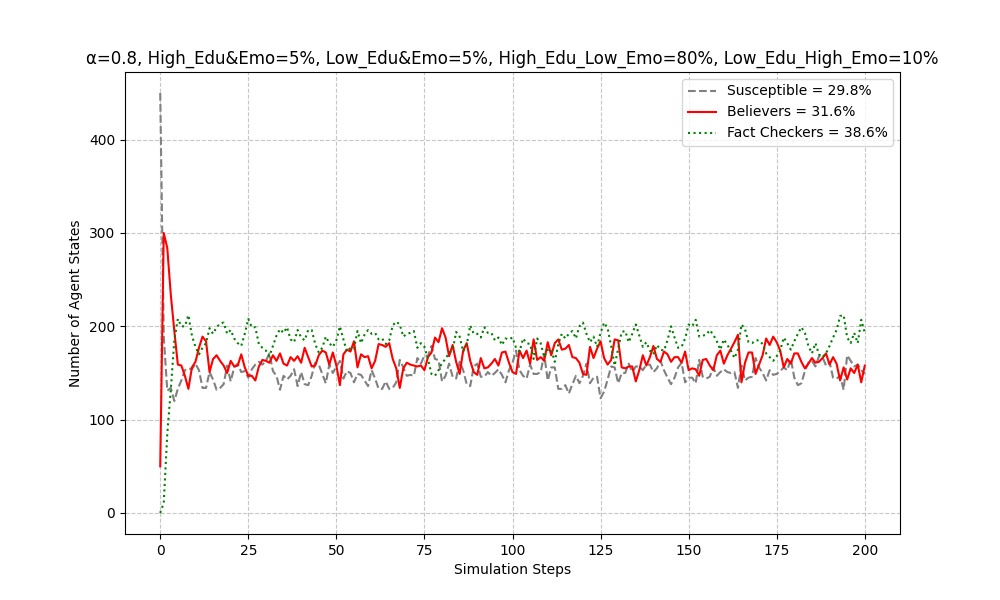
\includegraphics[width=1\linewidth]{high_alpha_min_threshold.png}
    \caption{Minimum threshold for fact checking, $\alpha$=0.8}
    \label{fig:8}
\end{figure}

Therefore, in order to limit the spread of misinformation and ensure that for any social network system of having more fact checkers than hoax believers. The above percentages of certain socio emotional classes needs to be present and maintained in this network or any subsequent subnetwork, according to the credibility value of the misinformation.

Fourthly, one interesting intervention technique, which is widely used on the popular "X" platform, is the community notes feature. It has been shown to increase the speed of fact checking according to the cited paper \cite{community_notes}.

This can be simulated in the project by adding initial fact checkers to the system, like the 10\% initial believers that are added to the network at the start, which should hypothetically heavily reduce the misinformation spread, and attain a lower minimum threshold for the high education with low emotion class.

When starting the network with fact checkers alongside believers and using a low hoax credibility (0.3), it has been observed that the minimum percentage for the high education with low emotional state class needed is at least 48\%, for the system to be mostly fact checkers and prevent it from becoming populated with misinformation believers, as can be seen in Figure \ref{fig:9}.

\begin{figure}[H]
    \centering
    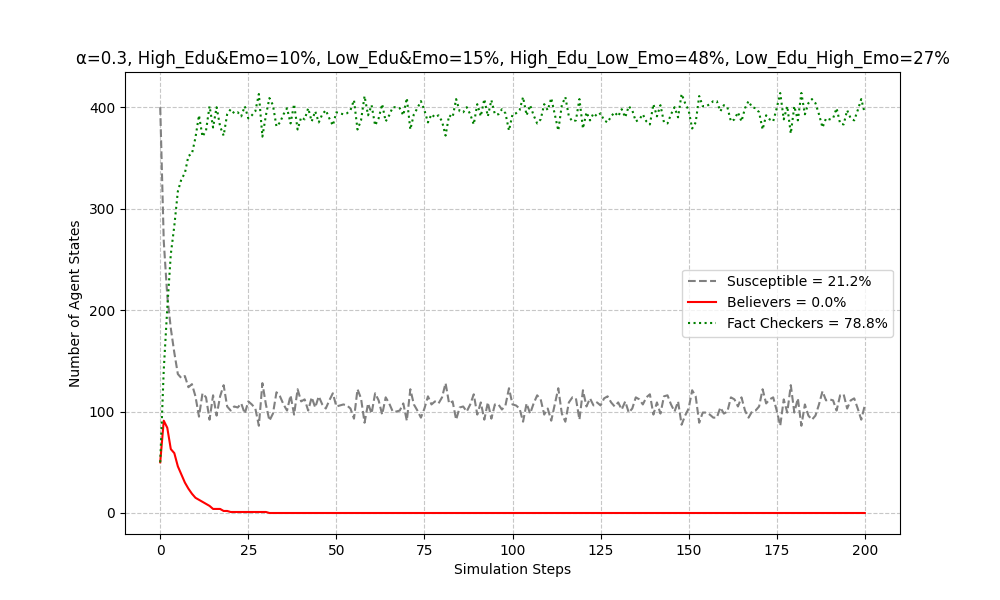
\includegraphics[width=1\linewidth]{intervention_low_alpha.png}
    \caption{Intervention Technique no.1, $\alpha$=0.3}
    \label{fig:9}
\end{figure}

When starting the network with fact checkers alongside believers and using a high hoax credibility (0.8), it has been observed that the minimum percentage for the high education with low emotional state class needed is at least 77\%, for the system to be mostly fact checkers and prevent it from becoming populated with misinformation believers, as can be seen from the below graph.



\section{Discussion}
First off, this experiment contributes to the larger research area of Artificial Life by modelling the spread of misinformation as a dynamic phenomenon in artificial social networks. Artificial life seeks to understand how alive beings behave and interact, by simulating this behaviour in an artificial system. This project aligns with the artificial life's goal by simulating how individual traits, such as education, anger, and trust influence behaviours of life like processes.

The agent based approach studies artificial populations, which is one of the main aspects of Artificial life, where simple agent-level rules lead to complex, system wide outcomes. Additionally, the project explores artificial societies, which is a subfield of artificial life, by examining socio emotional classes and their role in shaping information dissemination ecosystems. By providing valuable insights into how emotional and intellectual parameters drive the spread of misinformation, this work bridges the gap between artificial systems and real world societal challenges of false information spreading in a social network system, contributing to the understanding of life like processes in digital and computational environments.

The above results clearly show that a high education parameter does indeed increase the probability of an agent in the system to fact check, and decrease the probability of believing the misinformation, even in the case of a high credibility parameter. Thus proving that having a higher education level and media awareness, mitigate the spread of misinformation in a social network system, and cause other connections to be less susceptible to believe in this misinformation, as it can be observed from the model, that every agent is affected by all of his connections.

The same can be said about a high anger parameter, in terms that it increases the probability of any agent to be susceptible to believing a hoax without checking its validity.

It is clear that the intervention of introducing fact checkers into the system is successful. As the percentage of the high education with low emotional state class needed drops from 63\% to only 48\% when the hoax has a low credibility value, and a lower drop from 80\% to 77\% in the case of a hoax having a high credibility value. It is also worth mentioning that the effect of the fact checking intervention technique, is seen more strongly in the event that the hoax have a low credibility score, where a significant drop of 15\% was seen. But a much lower drop of only 3\% in the case of the hoax having a high credibility score.

Mitigating the spread of misinformation is very crucial, as spreading some misinformation (e.g. medical information) can cause the loss of human lives in the real world. This was the case in 2021 when false information were spread widely about the COVID-19 virus. Not only was false medical information about COVID-19 spread, but also bots were the ones who were spreading these false information \cite{covid}, so it was excessively spread as bots do not rest or sleep like humans do. That is why more advanced and modern intervention methods are needed more than even, as now two misinformation spreading frontiers are to be faced, humans and sleepless bots.

With the rise of artificial intelligence and its applications, one cited paper addressed using artificial intelligence to combat the spread of misinformation. The paper suggested incorporating a hybrid fact checking approach, using artificial intelligence in collaboration with humans. Following either a machine in a loop model, where human fact checkers generate final credibility warning labels based on AI model recommendations, or a human in the loop model, where artificial intelligence systems determine when to request human input. \cite{ai_detection}

But not all of modern artificial intelligence is good in combating the spread of misinformation, in fact it was stated by a cited paper that modern artificial intelligence applications, including generative artificial intelligence or Gen AI for short and large language models such as ChatGPT-4, Claude Sonnet, and Llama, are increasing the spread of medical and psychiatry misinformation, rather than help reducing it. \cite{ai_increasing_misinformation}

These modern artificial intelligence models generate content based on patterns in data while they were being trained, but these models lack true understanding and context of said data; which leads to errors, fabricated sources, and outputs that are biased towards a certain direction. Such misinformation, particularly in mental health, have the ability to put individuals and public health in danger. Public trust in AI is often misplaced due to limited education regarding technology, highlighting the urgent need for education, human supervision, and strategies to reduce misinformation while at the same time utilizing the benefits of such artificial intelligence models. \cite{ai_increasing_misinformation}

Another cited paper had the same results as the one above, where it explores how artificial intelligence can create highly credible looking misinformation, that is also hard to detect. The researchers used models like GPT-3, to generate fake content based on real COVID-19 misinformation, to later compare it with human made misinformation. They found that misinformation generated by AI often included emotional language, and human-like tones, thus making it more difficult to identify as fake. While existing detection models, like COVID-Twitter-BERT, can identify human-made misinformation well, they are less effective for AI generated content, due to its complexity and mix of truth and falsehood. Additionally, traditional methods for spotting misinformation, such as verifying the sources and searching for backing evidence, are less useful since AI misinformation often follows these credibility rules. The study highlights the need for new tools and strategies to detect and combat misinformation created by artificial intelligence systems. \cite{ai_increasing_misinformation_2}

Another cited paper explored strategies to try and mitigate the spread of viral misinformation, which was described as a significant societal issue impacting public health and democracy. Using a generative model, inspired by the dynamics of an infectious disease, the research paper analysed over 10.5 million tweets from the 2020 U.S. presidential election to evaluate effective interventions. These included fact checking, content removal, and virality circuit breakers (VCBs) to limit algorithmic amplification, nudges to encourage responsible sharing, and banning accounts for repeat offenders. While each individual intervention technique had its own limitations, it was discovered that by combining these approaches together, a significant reduction of well over 50\% to the spread of misinformation was observed, with more aggressive combinations of the above tactics achieving up to a reduction of 63\%. The study highlights the importance of multi-faceted strategies and calls for scalable solutions, addressing both practical and ethical challenges. \cite{reduce_misinformation}

This research can be further expanded by a multitude of ways, one way would be to explore a broader range of emotions beyond the emotional parameter that has been used in this study, which is anger. Frustration and stubbornness are a great example when it comes to studying other promising emotional parameters. By deeply tapping into these emotions, a far greater understanding of human behaviour and decision making can be gained, thus helping to understand its effect on spreading misinformation in social networks or even in real life.

Another way, is to introduce another set of logical parameters, such as critical thinking, reasoning, and problem solving skills. Studying these parameters closely could offer deeper insights and data into how people approach processing information, whether that's misinformation or truthful information. Another great direction would be to examine more exciting hybrid logical emotional parameters, such as hope and resilience.

Through looking at a wider range of emotional and cognitive variables, the research could offer a more comprehensive view of human dynamics, helping us to better understand how emotions and logic work hand in hand in shaping human behaviours, perceptions, and outcomes in various different situations and contexts. Which in turn helps in mitigating the spread of misinformation in both the real world and social networks, as the same human behaviour remains the same in both realms.


\section{Bibliography}
\printbibliography[heading=none]

\end{document}